\section{Auswertung}
\label{sec:Auswertung}
\subsection{Bestimmung der materialspezifischen Schallgeschwindigkeit}
Zur Bestimmung der materialspezifischen Schallgeschwindigkeit werden die
Durchlaufzeiten gegen die durchlaufene Strecke aufgetragen. Für das
Impuls-Echo-Verfahren gilt der Zusammenhang
\begin{equation*}
  h = \frac{1}{2} ct
\end{equation*}
für das Durchschallung-Verfahren der Zusammenhang
\begin{equation*}
  h = ct \; .
\end{equation*}
Aus den aufgetragenen Werten kann dann für das Impuls-Echo-Verfahren
eine Ausgleichsgerade mit der Form
\begin{equation*}
  t(h) = 2 \frac{h}{c} + \Delta t
\end{equation*}
berechnet werden. Für das Durchschallungsverfahren ergibt sich eine
Ausgleichgerade mit der Form
\begin{equation*}
  t(h) = \frac{h}{c} + \Delta t \; .
\end{equation*}
Alle Werte sind in den Tabellen \ref{tab:Tabs} dargestellt. Die Ausgleichsgeraden
mit Werten sind in den Abbildungen \ref{fig:IEplot} und \ref{fig:DSplot} dargestellt.
Der Ausdruck $ \Delta t$ in den Ausgleichsgeraden bezeichnet den systematischen
Fehler der aufgrund der Anpassungsschicht der Sonden entsteht. Aus der
Ausgleichsrechnung für das Impuls-Echo-Vefahren lässt sich dann entnehmen,
dass die materialspezifische Schallgeschwindigkeit
\begin{equation*}
  c_{IE} = \SI{2720(10)}{\meter\per\second}
\end{equation*}
und der systematische Fehler
\begin{equation*}
  \Delta t = \SI{3(2)e-7}{\second}
\end{equation*}
beträgt. Für das Durchschallungs-Verfahren ergeben sich die Werte
\begin{equation*}
  c_{DS} = \SI{2717(31)}{\meter \per \second}
\end{equation*}
für die Schallgeschwindigkeit und für den systematischen Fehler
\begin{equation*}
  \Delta t = \SI{1.3 (3)e-6}{\second}\; .
\end{equation*}
Im Mittel ergibt sich also für die Schallgeschwindigkeit in Acryl
\begin{equation*}
  \bar{c} = \SI{2718(16)}{\meter \per \second}
\end{equation*}
\begin{figure}
  \centering
  \caption{Werte des}
  \begin{subfigure}{0.48\textwidth}
    \caption{Impuls-Echo-Verfahren im Überblick.}
    \sisetup{round-mode = places, round-precision = 2}
    \begin{tabular}{S S}
      \toprule
      h / \si{\meter} & t / \si{\second} \\
      \midrule
      1.200600000000000001e-01 & 8.770000000000000397e-05\\
      1.020000000000000073e-01 & 7.506000000000000302e-05\\
      8.009999999999999065e-02 & 5.846999999999999415e-05\\
      4.003999999999999920e-02 & 2.907999999999999602e-05\\
      3.099999999999999978e-02 & 2.243999999999999860e-05\\
      1.110999999999999904e-01 & 8.137999999999999672e-05\\
      7.104000000000000592e-02 & 5.214999999999999367e-05\\
      \bottomrule
    \end{tabular}
    \label{tab:IE}
  \end{subfigure}
  \begin{subfigure}{0.48\textwidth}
    \caption{Durchschallungs-Verfahren im Überblick.}
    \sisetup{round-mode= places, round-precision = 2}
    \begin{tabular}{S S}
      \toprule
      h / \si{\meter} & t / \si{\second} \\
      \midrule
      1.200600000000000001e-01 & 4.518999999999999254e-05\\
      1.020000000000000073e-01 & 3.902999999999999731e-05\\
      8.009999999999999065e-02 & 3.080999999999999809e-05\\
      4.003999999999999920e-02 & 1.627999999999999998e-05\\
      3.099999999999999978e-02 & 1.232999999999999884e-05\\
      \bottomrule
    \end{tabular}
    \label{tab:DS}
  \end{subfigure}
  \label{tab:Tabs}
\end{figure}




\begin{figure}
  \centering
  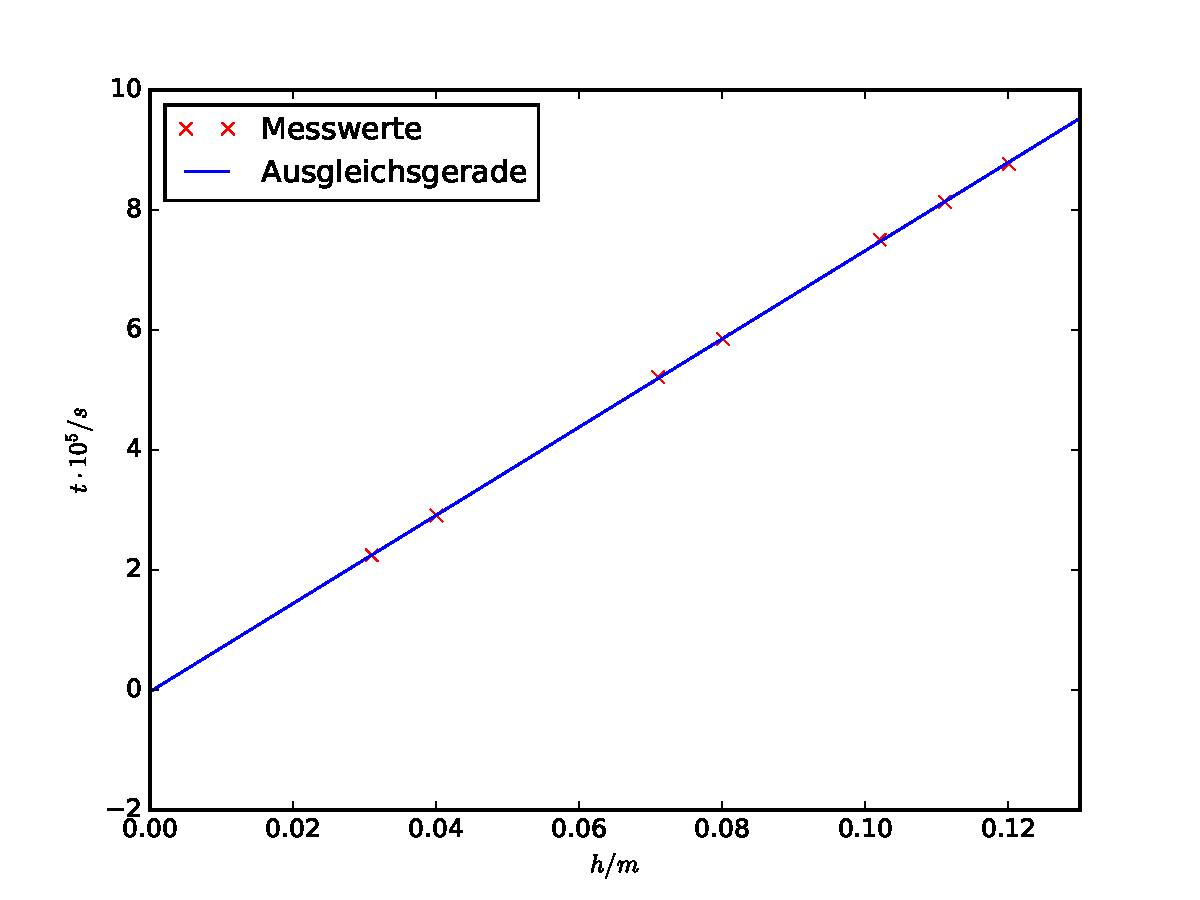
\includegraphics[height= 7cm]{plots/IE_plot.pdf}
  \caption{In diesem Diagramm wurde für das Impuls-Echo-Verfahren die Laufzeit des Ultraschallsignals gegen den "duchschallten" Weg aufgetragen. }
  \label{fig:IEplot}
\end{figure}
\begin{figure}
  \centering
  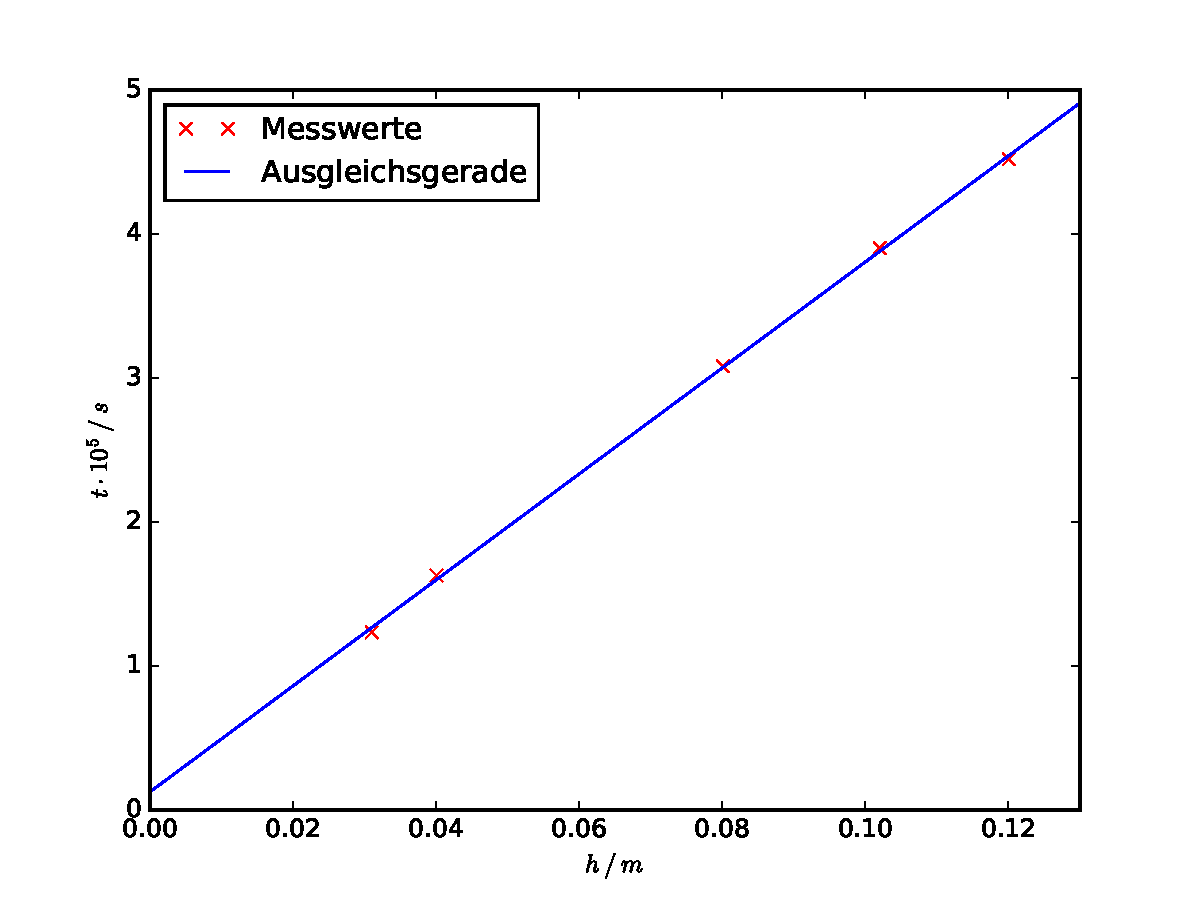
\includegraphics[height = 7cm]{plots/DS_plot.pdf}
  \caption{In diesem Diagramm wurde für das Durchsschallungs-Verfahren die Laufzeit des Ultraschallsignals gegen den "duchschallten" Weg aufgetragen. }
  \label{fig:DSplot}
\end{figure}
\FloatBarrier
\subsection{Bestimmung des materialspezifischen Schwächungskoeffizienten}
Zur Bestimmung des Schwächungskoeffizienten wird erst die Verstärkung $g$ von den Amplituden
abgerechnet, da folgender Zusammenhang gilt:
\begin{equation}
  g = 20 \cdot \symup{log}_{10}\left(\frac{I_v}{I_u}\right).
  \label{eqn:g}
\end{equation}
Dabei bezeichnet $I_u$ die unverstärkte und $I_v$ die verstärkte Amplitude.
Außerdem ist zu bemerken das nur die Amplitude $I_x$ verstärkt wurde.
Nun wird $ \symup{ln}\left(\sfrac{I_x}{I_0}\right)$ gegen $x$ aufgetragen,
dabei ist $x$ die doppelte Höhe der Zylinder. Die Ausgleichgerade kann nun mit
\begin{equation}
  \symup{ln}\left(\frac{I_x}{I_0}\right) = \alpha x
  \label{eqn:alph}
\end{equation}
berechnet werden. So ergibt sich für den Schwächungskoeffizient
\begin{equation*}
  \alpha = -\SI{21695(1524)}{\per\meter}\;.
\end{equation*}
Aus den Gleichungen \eqref{eqn:g} und \eqref{eqn:alph} ergibt sich der Zusammenhang
\begin{equation*}
  10^{\frac{gx}{20}} = \exp{\left(\alpha x \right)} \quad  \implies \quad g = \frac{20 \alpha}{\ln{\left(10 \right)}} \; ,
\end{equation*}
damit kann $\alpha$ in \si{\dB\per\meter} angegeben werden. Somit ergibt sich
\begin{equation*}
  \alpha = \SI{-1.9(1)e5}{\dB\per\meter} \; .
\end{equation*}
Alle Daten dazu sind in der Tabelle \ref{tab:alpha} und der Abbildung \ref{fig:alpha}
dargestellt.
\begin{table}
  \centering
  \caption{Werte zur Bestimmung des Schwächungskoeffizienten im Überblick}
  \sisetup{round-mode=places , round-precision= 2}
  \begin{tabular}{S S S S S}
    \toprule
    x / \si{\meter} & ln $\frac{I_x}{I_0}$& $I_{0}$/ \si{\volt}& $I_x$/\si{\volt}& Gain / dB \\
    \midrule
    2.401199999999999982e-04 & -5.243157530807446065e+00 & 1.314999999999999947e+00 & 2.020000000000000129e-01 & 2.926999999999999957e+01\\
    2.039999999999999984e-04 & -4.893557677756856350e+00 & 1.284999999999999920e+00 & 2.800000000000000266e-01 & 2.926999999999999957e+01\\
    1.601999999999999908e-04 & -3.424203187938578807e+00 & 1.284999999999999920e+00 & 1.217000000000000082e+00 & 2.926999999999999957e+01\\
    8.007999999999999223e-05 & -1.229715290417348283e+00 & 1.284999999999999920e+00 & 1.227000000000000091e+00 & 1.027999999999999936e+01\\
    6.200000000000000270e-05 & -4.640524218794533362e-01 & 1.284999999999999920e+00 & 1.002000000000000002e+00 & 1.870000000000000107e+00\\
    \bottomrule
  \end{tabular}
  \label{tab:alpha}
\end{table}
\begin{figure}
  \centering
  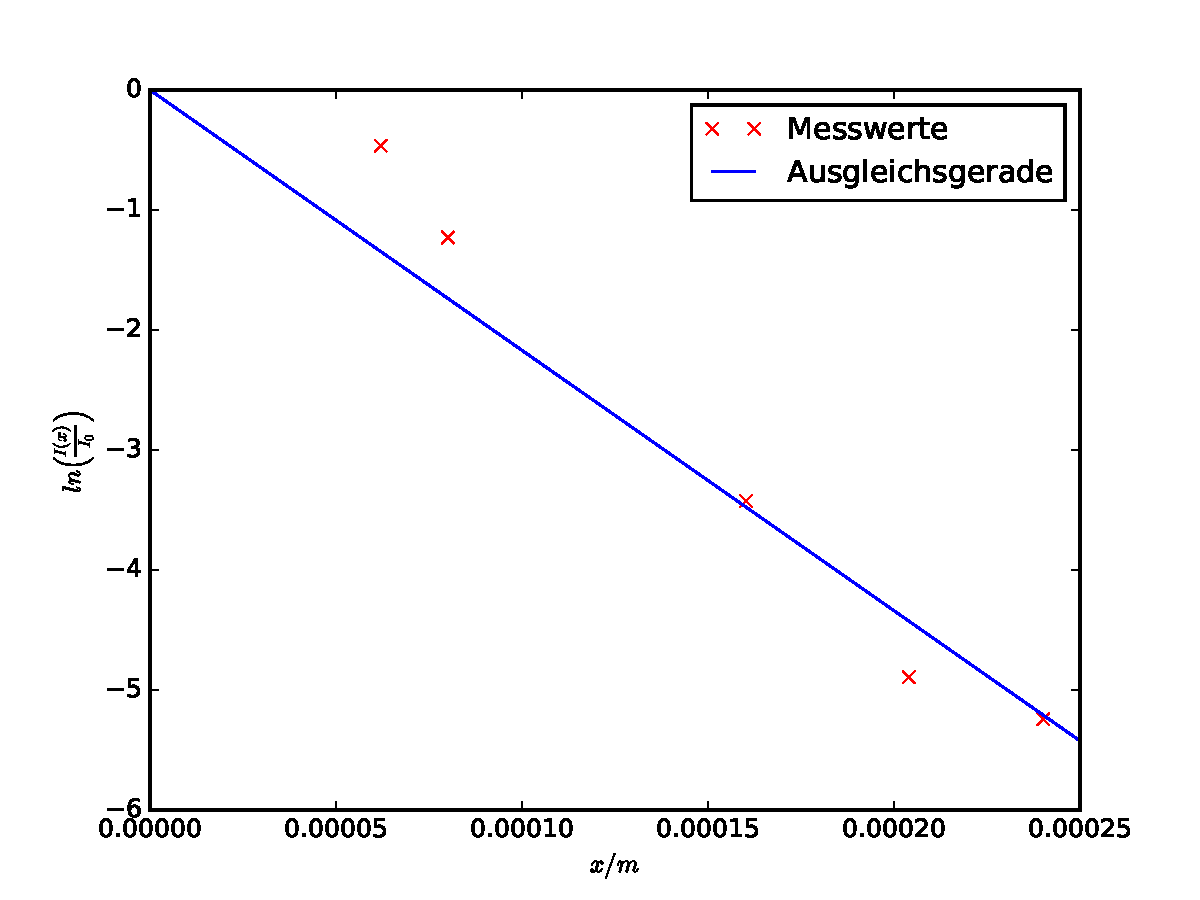
\includegraphics[height = 7cm]{plots/alphaplot.pdf}
  \caption{Ausgleichsgerade zur Bestimmung des Schwächungskoeffizienten}
  \label{fig:alpha}
\end{figure}

\FloatBarrier
\subsection{Spektrale Analyse}
Duch den Zusammenhang
\begin{equation*}
h = \frac{c}{2} t
\end{equation*}
können die Dicken der Blatten die mit dem Impuls-Echo-Verfahren durchleuchtet
wurden bestimmt werden. Aus der Abbildung \ref{fig:SA} werden die Positionen
der Echopeaks entnommen (s.Tabelle \ref{tab:SAW}), welche anzeigen wo bzw. wann der Ultraschall eine
Grenzfläche passiert. Somit verändert sich der Zusammenhang wie folgt:
\begin{equation*}
  h = \frac{\bar{c}}{2} \Delta t \; .
\end{equation*}
Das $\Delta t $ bezeichnet dabei den Zeitunterschied zwischen den Peaks.
Daraus ergibt sich dann, dass die erste Platte ca. \SI{5.43(3)}{\milli\meter}
und die zweite Platte ca. \SI{8.16(5)}{\milli\meter} dick ist.
\begin{table}
  \centering
  \caption{Aus Abbildung \ref{fig:SA} entnommene Werte}
  \begin{tabular}{c c}
    \toprule
    Peak & Depth  / \si{\micro\second}\\
    \midrule
    1 & 2 \\
    2 & 30 \\
    3 & 34 \\
    4 & 40 \\
    \bottomrule
  \end{tabular}
\label{tab:SAW}
\end{table}
\FloatBarrier
Im Vergleich zu den in den vorherigen Kapiteln bestimmten Werten sollte
der Abstand zwischen Peak 1 und 2 \SI{16.3}{\micro\second} betragen.

\begin{figure}
  \centering
  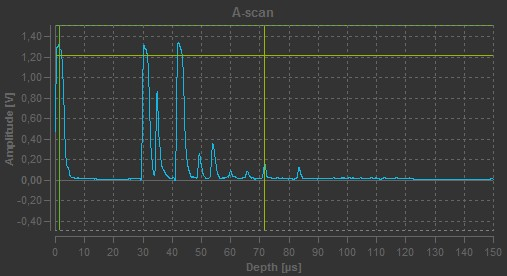
\includegraphics[height = 5cm]{FFS-Data/a_scan_spektrale_analyse.jpg}
  \caption{Spektrale Analyse von einem Acrylzylinder auf zwei unterschiedlich dicken Platten.}
  \label{fig:SA}
\end{figure}
\begin{figure}
  \centering
  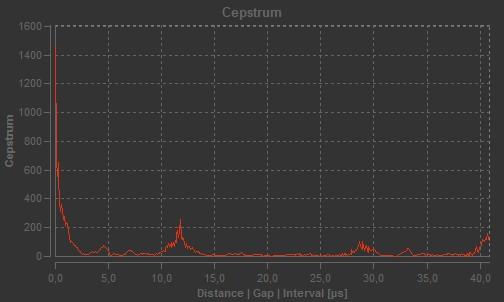
\includegraphics[height = 5cm]{FFS-Data/cepstrum_spektrale_analyse.jpg}
  \caption{Cepstrum von einem Acrylzylinder auf zwei unterschiedlich dicken Platten.}
  \label{fig:SAC}
\end{figure}
\subsection{Biometrische Untersuchung des Augenmodells}
Wie im Kapitel zuvor wird aus der Abbildung \ref{fig:AU} die Positionen der
Peaks bestimmt (s. Tabelle \ref{tab:AU}) und mit dem selben Zusammenhang wie zuvor die Abstände innerhalb
des Auges bestimmt. Hierbei ist doch zubeachten, dass es innerhalb des Auges
verschiedene Schallgeschwindgkeiten gibt. So beträgt die Schallgeschwindgkeit
in der Linse \SI{2500}{\meter\per\second} und in der Glaskörperflüssigkeit
\SI{1410}{\meter \per \second}.
Daraus ergibt sich dann für den Abstand zwischen Hornhaut und Linse
\SI{5.6}{\milli\meter} und für den Durchmesser der Linse \SI{3.7}{\milli\meter}.
Der Abstand zwischen Linse und Retina beträgt \SI{3.8}{\centi\meter}.

\begin{table}
  \centering
  \caption{Aus Abbildung \ref{fig:AU} entnommene Daten}
  \begin{tabular}{c c}
  \toprule
  Peak & Depth /\si{\micro \second} \\
  \midrule
  1 & 2 \\
  2 & 10 \\
  3 & 13 \\
  4 & 67 \\
  \bottomrule
\end{tabular}
\label{tab:AU}
\end{table}

\begin{figure}
  \centering
  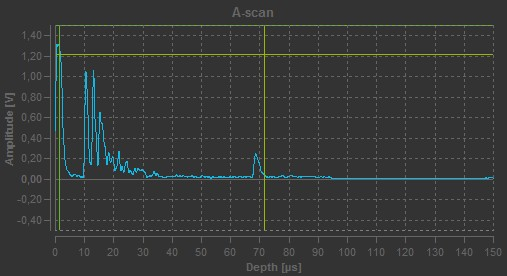
\includegraphics[height = 5cm]{FFS-Data/a_scan_auge.jpg}
  \caption{Spektrale Analyse des Augenmodells.}
  \label{fig:AU}
\end{figure}
